\chapter{Introduction to Probabilistic Learning}
\label{ch:intro}
\section{Introduction}
% \textcolor{red}{Motivation (including causality)}

Probabilistic learning means we {\bf model} our data  using probabilities. For example in classification, we aim to estimate the posterior probability of an item $x$: $p(c|x)$ for every possible class $c$. To develop complex probabilistic models, we will use basic concepts in probabilities such as the Bayes rule:
\begin{equation}
p(x,c) = p(x|c)p(c) \quad\Rightarrow\quad p(c|x) = \frac{p(x|c)p(c)}{\sum\limits_k p(x|k)p(k)}. \label{eq:bayes-rule} 
\end{equation}

But before that, we should quickly recall what do these "$p$" mean.
\begin{itemize}
 \item For {\bf discrete variables} (i.e.\ measurable events are discrete), the $p(c)$ is the probability that the random variable takes the value $c$, and we write:
\begin{equation} p(c) = P(C=c). \end{equation}
\item For {\bf continuous variables} (i.e.\ measurable events are continuous), $p(x)$ denotes the probability density function $f_X$ at $x$:
\begin{equation} p(x) = f_X(x) \end{equation}
and that probabilities can be computed over measurable sets, as the integral over the set:
\begin{equation} p({\cal X})=P(x\in{\cal X})=\int_{\cal X}f_X(x)\textrm{d}x. \end{equation}
As a consequence, the probability of a single value is always zero $P(\{x\})=0$.
\end{itemize}

We will be discussing probabilistic models with \textbf{hidden} or \textbf{latent} random variables. This means that some variables of the model will be observed, while other will not be observed (thus latent/hidden). This is useful for a wide variety of applications.

\paragraph{Example 1: Clustering} Given a set of data points $(x_j)_{j=1,\ldots,n}$ in ${\mathbb R}^d$, we aim to find (\& predict) clusters (groups of points). In a probabilistic model-based approach, we will have one latent variables assigned to each point, $z_j$. The realisation of the latent variable will index the cluster the associated observation belongs to. The model states that two observations belonging to the same cluster should have the same conditional distribution. We will discuss this model in detail in the Gaussian mixture model (GMM) chapter.
\begin{figure}[H]
\centering
\includegraphics[height=4.5cm]{fig/clustering-3.pdf}
\caption{Example of a clustering result in 2D with 3 clusters.}
\end{figure}


\paragraph{Example 2: Dimensionality Reduction} It is difficult to work with high-dimensional data (visualisation, pattern identification, etc). Ideally we would like to use a lower-dimensional representation. One possibility is to project in the subspace spanning the largest variance/energy. We will discuss more about this in the probabilistic principal component analysis (PPCA) chapter.
	
\begin{figure}[H]
\centering
\includegraphics[height=4.4cm]{fig/ppca_cloud_axes.pdf}
\caption{Example of dimensionality reduction result from 3 to 2 dimensions (spanned by the blue and red vectors. The original points are projected in the sub-space with lower dimension (e.g.\ green arrow).}
\end{figure}


\paragraph{Example 3: Analysis of Sequential Data} Temporal data segmentation can be seen as a special case of clustering, where temporal dependencies are important. One can hypothesize that the observation/latent variables at time $t$ depend only on a few of the past variables. In that case we say that the model is Markovian. A very important example are hidden Markov models (HMM), that will we widely discussed.
\begin{figure}[H]
\centering
\includegraphics[height=4.4cm]{fig/hmm.pdf}
\caption{Example of temporal segmentation of a time-series into three color-coded different segments.}
\end{figure}


In addition, we will also discuss approximate inference tools, mainly variational inference. In particular the family of variational autoencoders. We will also discuss other non-linear models such as normalising flows and diffusion models.



\section{Multivariate Gaussians}

\subsection{Recalling the 1D Gaussian Distribution}

% \begin{frame}{Quick reminder}
Let's recall the definition of the probability density function of \textbf{univariate Gaussian distribution}:
\begin{equation}
p(x) = \mathcal{N}(x;\mu,\nu) = \frac{1}{\sqrt{2\pi\nu}}\exp\Big(-\frac{(x-\mu)^2}{2\nu}\Big), 
\end{equation}
with $x\in\mathbb{R}$, $\mu\in\mathbb{R}$ and $\nu\in\mathbb{R}^{+}$. The parameters $\mu$ and $\nu$ are called respectively the mean and the variance, and satisfy:
\begin{equation}
 \mu = \mathbb{E}_{p(x)}\{x\} \qquad \nu = \mathbb{E}_{p(x)}\{(x-\mu)^2\}.
\end{equation}

\remark{definition-expectation}{We will often use the \textbf{expectation} of a function $f$ of a random variable $x$ w.r.t.\ the probability density function $p(x)$, and denote it by:
\begin{equation}
 \mathbb{E}_{p(x)}\{f(x)\} = \int_{\mathcal{X}} f(x)p(x)\textrm{d}x,
\end{equation}
where $\mathcal{X}$ is the domain of the random variable $x$.}

One very common and useful concept is the maximum-likelihood estimators. To derive them, we assume the existence of $N$ observations $X=\{x_1,\ldots,x_N\}$ following a univariate Gaussian distribution, and the aim is to find the values of the parameters maximising the log-likelihood:
\begin{equation}
\mathcal{L}(\mu,\nu|X) = \sum_{n=1}^N \log \mathcal{N}(x_n;\mu,\nu)
\end{equation}

\exercise{ml-uni-gaussian}{Prove that the expressions for the maximum likelihood estimators $\mu^*$ and $\nu^*$ are:
\begin{equation}
\mu^* = \frac{1}{N}\sum_{n=1}^N x_n \qquad \nu^*=\frac{1}{N}\sum_{n=1}^N (x_n-\mu^*)^2.
\end{equation}}

\subsection{Constructing Multivariate Gaussian Distributions}

\paragraph{As Product of Independent Gaussians} But what happens now if we want to define a Gaussian on $\mathbb{R}^D$? One trivial extension of the 1D Gaussian is to consider each dimension as an independent Gaussian, with a different mean and variance: $\mu_1,\ldots,\mu_D$ and $\nu_1,\ldots,\nu_D$.
 
In that case the density writes:
\begin{equation}
p(\mathbf{x}) = \mathcal{N}(\mathbf{x};\bs{\mu},\bs{\nu}) = \prod_{d=1}^D\frac{1}{\sqrt{2\pi\nu_d}}\exp\Big(-\frac{(x_d-\mu_d)^2}{2\nu_d}\Big),
\end{equation}

where we have defined $\mathbf{x}=(x_1,\ldots,x_D)\in\mathbb{R}^D$, $\bs{\mu}=(\mu_1,\ldots,\mu_D)\in\mathbb{R}^D$ and $\bs{\nu}=(\nu_1,\ldots,\nu_D), \nu_d\in\mathbb{R}^{+}$.

\begin{figure}[H]
 \centering
 \includegraphics[width=0.5\textwidth]{fig/multivariate_gaussian}
 \caption{Probability density function of a 2D Gaussian distribution.}
 \label{fig:pdf-2d-Gaussian}
\end{figure}

\exercise{ml-orth-gaussian}{Derive the maximum likelihood estimators for $\bs{\mu}$ and $\bs{\nu}$.} 

This is a special case of a multivariate Gaussian distribution. To present the more general case, we first remark that the above expression can be rewritten using matrix notation. Indeed, by defining:
\begin{equation}
    \bs{\Sigma}=\textrm{diag}(\boldsymbol{\nu})=\left(\begin{array}{cccc}
    \nu_1 & 0 & \ldots & 0 \\
    0 & \nu_2 & \ldots & 0 \\
    \vdots & \vdots & \ddots & \vdots \\
    0 & 0 & \ldots & \nu_D
    \end{array}\right)
\end{equation}
the density rewrites as:
\begin{equation}
    p(\mathbf{x}) = \mathcal{N}(\mathbf{x};\bs{\mu},\bs{\Sigma}) = \frac{1}{\sqrt{|2\pi\bs{\Sigma}|}}\exp\Big(-\frac{1}{2}(\bs{x}-\bs{\mu})^\top\bs{\Sigma}^{-1}(\bs{x}-\bs{\mu})\Big).
\end{equation}
\exercise{matrix-form-equivalence-gaussian}{Prove it!}
 
\paragraph{Generalisation to ``any'' Covariance Matrix} Naturally, the question of the constraints/conditions on the matrix $\bs{\Sigma}$ arises. In other words, one wonders whether or not a multivariate Gaussian distribution can be defined for any matrix $\bs{\Sigma}$. The answer is simply no. The so-called \textbf{covariance matrix} must be  \textit{symmetric} and \textit{positive definite} matrices.\vspace{2mm}
 
\remark{positive-definite}{A $D\times D$ symmetric matrix $\bs{\Sigma}$ is \textbf{positive definite} if and only if $\bs{v}^\top\bs{\Sigma}\bs{v} > 0$, $\forall \bs{v}\neq \bs{0}$.}

For the Gaussian distribution, this is intuitive, since the variance should be strictly positive in any direction, see Figure~\ref{fig:pdf-2d-Gaussian}. Let $\bs{\Sigma}$ be a symmetric and positive definite matrix, the $\bs{\Sigma}$ has the following properties:
\begin{itemize}
    \item All eigenvalues of $\bs{\Sigma}$ are real and  strictly positive.
    \item The inverse of $\bs{\Sigma}$ is symmetric and positive definite.
    \item We can write $\bs{\Sigma}=\bs{U}\bs{\Lambda}\bs{U}^\top$ with $\bs{\Lambda}$ diagonal and $\bs{U}$ orthogonal, with $\bs{\Lambda}$ containing the eigenvalues and $\bs{U}$ the eigenvectors (as columns).
    \item With this notation the inverse writes: $\bs{\Sigma}^{-1} = \bs{U}\bs{\Lambda}^{-1}\bs{U}^\top$.
\end{itemize}

\exercise{inv-pdf-matrix}{Prove that the inverse of a (symmetric) positive definite matrix always exists.}

If $\bs{\Sigma}$ is a covariance matrix we can define the \textit{Mahalanobis} distance:
\begin{equation}
\mathcal{M}(\bs{x};\bs{\mu},\bs{\Sigma}) = (\bs{x}-\bs{\mu})^\top\bs{\Sigma}^{-1}(\bs{x}-\bs{\mu})
\end{equation}
(which is the Euclidean distance for $\bs{\mu}=\bs{0}$ and $\bs{\Sigma}=\bs{I}$).\\

\remark{def-mv-Gaussian}{Given a vector $\bs{\mu}\in\mathbb{R}^D$ and symmetric and positive definite matrix $\bs{\Sigma}\in\mathbb{R}^{D\times D}$, we can define the probability density function of a \textbf{multivariate Gaussian} distribution as:
\begin{equation}
\mathcal{N}(\bs{x};\bs{\mu},\bs{\Sigma}) = \frac{1}{\sqrt{|2\pi\bs{\Sigma}|}}\exp\Big(-\frac{1}{2}\mathcal{M}(\bs{x};\bs{\mu},\bs{\Sigma})\Big) = \frac{1}{\sqrt{|2\pi\bs{\Sigma}|}}\exp\Big(-\frac{1}{2}(\bs{x}-\bs{\mu})^\top\bs{\Sigma}^{-1}(\bs{x}-\bs{\mu})\Big)
\end{equation}
}

The vector $\bs{\mu}$ and the matrix $\bs{\Sigma}$ are usually referred to as the \textit{mean vector} and the \textit{covariance matrix}. The covariance matrix corresponds to the variance (and not to the standard deviation) of a univariate Gaussian. Formally, the mean vector and covariance matrix are defined as:
\begin{equation}
 \bs{\mu} = \mathbb{E}_{\mathcal{N}(\bs{x};\bs{\mu},\bs{\Sigma})}\{\mathbf{x}\} \qquad \bs{\Sigma} = \mathbb{E}_{\mathcal{N}(\bs{x};\bs{\mu},\bs{\Sigma})}\{(\mathbf{x}-\bs{\mu})(\mathbf{x}-\bs{\mu})^\top\}.
\end{equation}


\exercise{norm-mv-Gaussian}{Prove that the normalisation constant of a multivariate Gaussian distribution with covariance matrix $\bs{\Sigma}$ is $\sqrt{|2\pi\bs{\Sigma}|}$.}

\paragraph{As Linear Transformations of the Standard Gaussian} Multivariate Gaussian distributions can be constructed from the so-called standard Gaussian by using linear transformations.\vspace{2mm}

\remark{standard-gaussian}{The standard multivariate Gaussian is defined as the zero-mean and unit-variance Gaussian distribution, or equivalently, as the cartesian product of $D$ univariate standard Gaussian distributions. The associated probability density function writes:
\begin{equation}
 \mathcal{N}(\mathbf{z};\mathbf{0},\mathbf{I}) = \frac{1}{(2\pi)^{D/2}}\exp\Big(-\frac{1}{2}\|\mathbf{z}\|^2\Big).
\end{equation}
}\vspace{2mm}

\exercise{mv-gaussian-linear-construction}{Let us consider the case where $\mathbf{z}$ follows a standard multivariate Gaussian distribution, and we define $\mathbf{x}=\mathbf{A}\mathbf{z}+\bs{\mu}$ with $\mathbf{A}\in\mathbb{R}^{D\times D}$ being an invertible matrix ($|\mathbf{A}|\neq 0$). Prove that:
\begin{equation}
 p(\mathbf{x}) = \mathcal{N}(\bs{x};\bs{\mu},\bs{\Sigma}), \quad \text{with} \quad \bs{\Sigma} = \mathbf{A}\mathbf{A}^\top.
\end{equation}
}

Implicitly, we are saying that for any invertible matrix $\mathbf{A}$, $\mathbf{A}\mathbf{A}^\top$ is symmetric (obvious) and positive definite. We will use this construction using linear transformations to better understand multivariate Gaussians. We will take several particular cases, and plot the level curves and associated probability density functions. For plotting purposes we will restrict to $D=2$. For simplicity and without loss of generality, we will ignore the mean vector. We will consider four cases:
\begin{equation}
\mathbf{x} = \mathbf{z} \qquad\qquad \mathbf{x} = \underbrace{\left(\begin{array}{cc}\sqrt{2} & 0\\0 & 1/\sqrt{3}\end{array}\right)}_{\mathbf{A}_1}\mathbf{z} \qquad\qquad \mathbf{x} = \underbrace{\left(\begin{array}{cc}\cos(\theta) & -\sin(\theta)\\\sin(\theta) & \cos(\theta)\end{array}\right)}_{\mathbf{A}_2(\theta),\; \theta=30^\circ}\mathbf{z} \qquad\qquad \mathbf{x} = \mathbf{A}_2\mathbf{A}_1\mathbf{z}.
\end{equation}

The first case corresponds to plot the standard Gaussian:
\begin{figure}[H]
 \centering
 \includegraphics[width=0.7\textwidth]{fig/mv-gaussian-standard.png}
 \caption{Plots corresponding to the standard multivariate Gaussian. (left) Level curves and sample data points in green. (right) 3D plot of the probability density function, and associated level curves.}
\end{figure}

The second case corresponds to scaling the points with different values on the first and second dimension.
\begin{figure}[H]
 \centering
 \includegraphics[width=0.7\textwidth]{fig/mv-gaussian-scale.png}
 \caption{Plots corresponding to the standard multivariate Gaussian scaled using $\mathbf{A}_1$.}
\end{figure}

The third case will have the same plot as the first one, except that the samples will be rotated. The fourth case corresponds to composing scaling the rotation.
\begin{figure}[H]
 \centering
 \includegraphics[width=0.7\textwidth]{fig/mv-gaussian-full.png}
 \caption{Plots corresponding to the standard multivariate Gaussian scaled using $\mathbf{A}_2\mathbf{A}_1$.}
\end{figure}

It is clear now that for every invertible matrix we can obtain a different Gaussian distribution. Because of the decomposition of positive definite matrices into $\bs{\Sigma}=\mathbf{U}\bs{\Lambda}\mathbf{U}^\top$ discussed before, we can also see that every Gaussian distribution corresponds to a linear transformation of the standard Gaussian distribution. Indeed, we can simply consider the entry-wise squared-root of $\bs{\Lambda}$, $\mathbf{L}=\bs{\Lambda}^{1/2}$ and define $\mathbf{A}=\mathbf{U}\mathbf{L}$, then $\bs{\Sigma}=\mathbf{A}\mathbf{A}^\top$, and $\mathbf{A}$ is the linear (invertible) transformation applied to the standard normal.

We can state further properties of the multivariate Gaussian distribution regarding its level curves, defined as:
\begin{equation}
\mathcal{C}_\lambda = \{\bs{x}|\mathcal{N}(\bs{x};\bs{\mu},\bs{\Sigma})=\lambda\}. 
\end{equation}
These level curves are:
\begin{itemize}
    \item For $\lambda<0$, $\mathcal{C}_\lambda = \emptyset$.
    \item For $\lambda=0$, $\mathcal{C}_0=\{\bs{\mu}\}$.
    \item For $\lambda>0$, $\mathcal{C}_\lambda$? is an ellipsoid with center $\bs{\mu}$, axis given by the columns of $\bs{U}$ and axis length given by the elements in $\bs{\Lambda}$, where $\bs{\Sigma}=\bs{U}\bs{\Lambda}\bs{U}^\top$. See the figures above.
\end{itemize}

\subsection{Properties of Multivariate Gaussians}

\paragraph{Deriving Maximum Likelihood Estimators for Multivariate Gaussians} In order to derive maximum likelihood estimators for the parameters of the multivariate Gaussian distribution, we need to know how to take derivatives w.r.t.\ vectors and matrices. We will use some results from the matrix cookbook~\cite{matrix-cookbook}. Useful formulae:
\begin{equation}
\frac{\partial \textrm{Tr}(\bs{M}\bs{A})}{\partial\bs{M}}=\bs{A}^\top \qquad \frac{\partial \textrm{Tr}(\bs{B}^\top\bs{M}^\top\bs{C}\bs{M}\bs{B})}{\partial\bs{M}}=\bs{C}^\top\bs{M}\bs{B}\bs{B}^\top+\bs{C}\bs{M}\bs{B}\bs{B}^\top
\end{equation} 
\begin{equation}
\frac{\partial \log|\bs{M}|}{\partial\bs{M}}=(\bs{M}^{-1})^\top \qquad [\textrm{Tr}(\bs{A}\bs{B}\bs{C}) = \textrm{Tr}(\bs{B}\bs{C}\bs{A}) = \textrm{Tr}(\bs{C}\bs{A}\bs{B})]
\end{equation}

\exercise{ml-estimators-mv-gaussian}{Prove that the ML estimators of the multivariate Gaussian are:
\begin{equation}
\bs{\mu}^*=\frac{1}{N}\sum_{n=1}^N\bs{x}_n\qquad \bs{\Sigma}^* = \frac{1}{N}\sum_{n=1}^N (\bs{x}_n-\bs{\mu}^*)(\bs{x}_n-\bs{\mu}^*)^\top.
\end{equation}
}

\paragraph{The shape is all you need} $ $\\

\remark{shape-gaussians}{By developing the expression of the multivariate Gaussian distribution:
\begin{equation}
 \mathcal{N}(\bs{x};\bs{\mu},\bs{\Sigma}) = \frac{1}{\sqrt{|2\pi\bs{\Sigma}|}}\exp\Big(-\frac{1}{2}(\bs{x}-\bs{\mu})^\top\bs{\Sigma}^{-1}(\bs{x}-\bs{\mu})\Big) \stackrel{\mathbf{x}}{\propto} \exp\Big(-\frac{1}{2}\bs{x}^\top\bs{\Sigma}^{-1}\bs{x} + \bs{x}^\top\bs{\Sigma}^{-1}\bs{\mu}\Big),
\end{equation}
we observe that only two terms depend on $\mathbf{x}$. Both are in the exponential: one is quadratic and the other is linear.}

The notation $\stackrel{\mathbf{x}}{\propto}$ means that is proportional up to a constant that does NOT depend on $\mathbf{x}$. This notation will be very useful along these notes. In other words, as long as the shape of the distribution is exponential with a quadratic and a linear term on the random variable, then the distribution is Gaussian. The only constraint is that the quadratic term must have negative signe and the matrix should be symmetric and positive definite.\vspace{2mm}

\exercise{gaussian-completion}{Prove that given a symmetric and positive definite matrix $\bs{\Omega}$ and a vector $\mathbf{m}$, a probability distribution of the form:
\begin{equation}
 p(\mathbf{x}) \stackrel{\mathbf{x}}{\propto} \exp\Big(-\frac{1}{2}\mathbf{x}^\top\bs{\Omega}\mathbf{x} + \mathbf{x}^\top\mathbf{m}\Big)
\end{equation}
corresponds to a multivariate Gaussian distribution with the following covariance matrix and mean vector:
\begin{equation}
 \bs{\Sigma} = \bs{\Omega}^{-1} \qquad \qquad \bs{\mu} = \bs{\Sigma}\mathbf{m} = \bs{\Omega}^{-1}\mathbf{m}.
\end{equation}
}

More on multivariate Gaussians in Chapter~\ref{ch:ppca}.

\section{Latent Variables and Conditional Independence}
\subsection{Introduction}
We will be using \textit{models} between variables. In our case this model describes the relationships between two or more variables, see Figure~\ref{fig:simple-model}. In practice this means that we choose:
\begin{itemize}
    \item the nature of $\mathbf{z}$ \& $\mathbf{x}$: cont./discrete, bounded, ...
    \item the \textcolor{green}{dependencies}, i.e.\ $p(\mathbf{x},\mathbf{z})=p(\mathbf{x}|\mathbf{z})p(\mathbf{z})$.
    \item the \textcolor{red}{prior distribution} $p(\mathbf{z})$.
    \item the \textcolor{blue}{likelihood distribution} $p(\mathbf{x}|\mathbf{z})$.
\end{itemize}

%%% TODO Make it tikz
\begin{figure}[H]
 \centering
 \includegraphics[width=0.05\textwidth]{fig/simple-model.pdf}
 \caption{Simple model with two variables.\label{fig:simple-model}}
\end{figure}

\remark{latent-variable-def}{For the rest of the courses, we will make the difference between \textbf{observed} and \textbf{latent} or hidden variables. Observed variables are the samples obtained via measuring a system, and latent variables are quantities that cannot be measured directly.}

For instance, in the clustering task, the observations are the positions of the data points in the $\mathbb{R}^D$ space (measured), and the latent variables are the class index of each of the samples (not observed). Usually, $\mathbf{x}$ will denote the observation variable and $\mathbf{z}$ the hidden or latent variable.\vspace{2mm}
   
\remark{classical-questions}{The two classical questions in probabilistic models with latent variables, once the prior and likelihood distributions are defined are the \textbf{marginal distribution} of $\mathbf{x}$ (left) and the \textbf{posterior distribution} of $\mathbf{z}$ given $\mathbf{x}$ (right):
\begin{equation}
p(\mathbf{x}) = \displaystyle\int_{\cal Z} p(\mathbf{x}|\mathbf{z})p(\mathbf{z}) \textrm{d}\mathbf{z} \qquad\qquad  
p(\mathbf{z}|\mathbf{x}) = \displaystyle\frac{p(\mathbf{x}|\mathbf{z})p(\mathbf{z})}{p(\mathbf{x})}
\end{equation}
}

Formally, both $p(\mathbf{z})$ and $p(\mathbf{x})$ are marginal distributions. Because of the sense of the dependency, the former is referred to as the marginal, while the latter as the prior. The same happens with $p(\mathbf{z}|\mathbf{x})$ and $p(\mathbf{x}|\mathbf{z})$: both are conditional or posterior distributions, but their name is different because of the sense of the dependency.

\paragraph{Example: Gaussian Mixture Model} The one-dimensional Gaussian mixture model (GMM) can be defined as follows:
\begin{itemize}
\item The nature: $z$ is discrete \& bounded, $x$ is 1D \& continuous.
\item The dependencies are: $p(x,z)=p(x|z)p(z)$.
\item The prior distribution $p(z)$, $z\in\{1,\ldots,K\}$ is categorical:
\begin{equation}p(z=k) = \pi_k, \qquad \pi_k\geq 0,\; \sum_{k=1}^K \pi_k = 1.\end{equation}
\item The likelihood distribution $p(x|z)$ is Gaussian:
\begin{equation}p(x|z=k) = {\cal N}(x;\mu_k,\nu_k) = \frac{1}{\sqrt{2\pi\nu_k}}\exp\Big(-\frac{(x-\mu_k)^2}{2\nu_k}\Big)\end{equation}
with $\mu_k\in\mathbb{R}$ and $\nu_k>0$, $\forall k$.
\end{itemize}

\exercise{1d-gmm-marginal}{Prove that given the prior and likelihood distributions of the GMM, the marginal writes:
\begin{equation}
 p(x) = \sum_{k=1}^K \pi_k \frac{1}{\sqrt{2\pi\nu_k}}\exp\Big(-\frac{(x-\mu_k)^2}{2\nu_k}\Big).
\end{equation}
}

\exercise{1d-gmm-posterior}{Prove that given the prior and likelihood distribution of the GMM, the posterior writes:
\begin{equation}
 p(z=k|x) = \frac{\pi_k \frac{1}{\sqrt{2\pi\nu_k}}\exp\Big(-\frac{(x-\mu_k)^2}{2\nu_k}\Big)}{\sum_{m=1}^K \pi_m \frac{1}{\sqrt{2\pi\nu_m}}\exp\Big(-\frac{(x-\mu_m)^2}{2\nu_m}\Big)}.
\end{equation}
}


 More on this on the Chapter~\ref{ch:gmm}.
% \end{frame}

\subsection{Conditional Independence}

% \subsection{3-variable models}

We will start study conditional independence with the smallest model that can be used: 3 variables. There are four types of 3-variable models, as depicted in Figure~\ref{fig:3-var-models}:
\begin{description}
    \item[Full] all dependencies are set:
    \begin{equation}
    p(x,y,z) = p(z|x,y)p(y|x)p(x)
    \end{equation}
    \item[Two-kids] $y\rightarrow z$ dependency missing:
    \begin{equation}
    p(x,y,z) = p(z|x{\color{lightgray},y})p(y|x)p(x)
    \end{equation}
    \item[Two-parents] $x\rightarrow y$ dependency missing:
    \begin{equation}
    p(x,y,z) = p(z|x,y)p(y{\color{lightgray}|x})p(x)
    \end{equation}
    \item[Cascaded] $x\rightarrow z$ dependency missing:
    \begin{equation}
    p(x,y,z) = p(z|{\color{lightgray}x,}\ y)p(y|x)p(x)
    \end{equation}
\end{description}

%% TODO: Pass to tikz
\begin{figure}[H]
\centering
\includegraphics[width=.15\textwidth]{fig/full-xyz.pdf}\hspace{1cm}
\includegraphics[width=.15\textwidth]{fig/twokids-xyz.pdf}\hspace{1cm}
\includegraphics[width=.15\textwidth]{fig/twoparents-xyz.pdf}\hspace{1cm}
\includegraphics[width=.15\textwidth]{fig/cascaded-xyz.pdf}
\caption{Three-variable models, from left to right: Full (all dependencies are used), Two-kids ($y\rightarrow z$ dependency missing), Two-parents ($x\rightarrow y$ dependency missing) and Cascaded ($x\rightarrow z$ dependency missing).\label{fig:3-var-models}}
\end{figure}

We will let aside the Full model, since we are interested in understanding the imapct of the missing dependencies. Let's analyse the Two-kids model in depth.\vspace{3mm}

\exercise{two-kinds-independence}{Prove that in the Two-kids model:
\begin{equation}
 p(y|z)\neq p(y) \qquad \text{and} \qquad  p(y|z,x) =  p(y|x)
\end{equation}
}\vspace{2mm}

The first statement is equivalent to say that $y$ and $z$ are not independent. The second statement, however, says that $y$ and $z$ are \textbf{conditionally independent} w.r.t.\ $x$. Let us repeat a similar analysis with the Two-parents model.\vspace{2mm}

\exercise{two-parents-independence}{Prove that in the Two-parents model:
\begin{equation}
 p(y|x) = p(x) \qquad \text{and} \qquad p(x|y,z) \neq p(x|z).
\end{equation}
}\vspace{2mm}

We are in the opposite case. The first statement says that $y$ and $x$ are independent, while the second statement says that $y$ and $x$ are conditionally dependent w.r.t.\ $z$. We will repeat this analysis for the Cascaded model.\vspace{2mm}

\exercise{cascaded-independence}{Prove that in the Cascaded model:
\begin{equation}
 p(x,z)\neq p(x)p(z) \qquad\text{and}\qquad p(x,z|y) = p(x|y)p(z|y).
\end{equation}
}\vspace{2mm}

In this case, we obtain similar results than with the Two-kids model.\vspace{3mm}

\remark{ind-vs-cond-ind}{At this point it should be clear that independence and conditional independence are \textbf{two very different properties} of random variables.}

\remark{cond-ind-definition}{
Let $x$, $y$, and $z$ be random variables, we say that $x$ and $y$ are \textbf{conditionally independent} given $z$, and write $x\indep y \;|\; z$, iff one of the following equivalent expressions holds:
\begin{itemize}
 \item $p(x,y|z) = p(x|z)p(y|z)$
 \item $p(x|y,z) = p(x|z)$
 \item $p(y|x,z) = p(y|z)$
\end{itemize}
}

\subsection{D-separation}
Let's consider the following variables and dependencies.
\begin{center}
\includegraphics[width=0.4\textwidth]{fig/huge-muvar.pdf}
\end{center}
Is $P \indep V \;|\; T$ ? How would you do it ? Is the previous strategy scalable ? Let us recall the 3-variable models:

\begin{figure}[H]
\centering
\includegraphics[width=0.15\textwidth]{fig/twokids-abc-color.pdf}\hspace{1cm}\includegraphics[width=0.15\textwidth]{fig/cascaded-abc-color.pdf}\hspace{2cm}\includegraphics[width=0.15\textwidth]{fig/twoparents-abc-color.pdf}
\caption{Recalling the 3-variable models with new variable names. From left to right: two-kids, cascaded and two-parents.\label{fig:3-var-highlighted}}
\end{figure}
\begin{description}
 \item[Two-kids] The path from $a$ to $b$ is called ``tail-to-tail.''
  \begin{equation}p(a,b|{\color{mypurple}c}) = p(a|{\color{mypurple}c})p(b|{\color{mypurple}c}) \end{equation}
 \item[Cascaded] The path from $a$ to $b$ is called ``head-to-tail.''
  \begin{equation}p(a,b|{\color{mypurple}c}) = p(a|{\color{mypurple}c})p(b|{\color{mypurple}c})\end{equation} 
 \item[Two-parents] The path from $a$ to $b$ is called ``head-to-head.''
  \begin{equation}p(a,b|{\color{mypurple}c}) \neq p(a|{\color{mypurple}c})p(b|{\color{mypurple}c})\end{equation}  
\end{description}

$\Rightarrow$ If $A \indep B \,|\, C$, nodes within tail-to-tail or head-to-tail can be in $C$ and nodes within head-to-head or any of their descendents must not be in $C$.\vspace{2mm}

\remark{blocked-path}{Let $A$, $B$ and $C$ be three non-intersecting sets of nodes of a directed acyclic graph. A path from $A$ to $B$ is said to be \textbf{blocked} by $C$ if it includes a node that either:
\begin{itemize}
\item the path meets tail-to-tail or head-to-tail at the node and the node is in C;
\item the path meets head-to-head at the node and neither the node nor any of its descendants are in C.
\end{itemize}}

\exercise{path-blocking}{Regarding the graphical model in Figure~\ref{fig:path-blocking}, please answer the following questions:
\begin{enumerate}
 \item Is the path from $\{x\}$ to $\{v\}$ blocked by $\{u\}$?
 \item Is the path from $\{x\}$ to $\{v\}$ blocked by $\{y\}$?
 \item Is the path from $\{x\}$ to $\{v\}$ blocked by $\{z\}$?
 \item Is the path from $\{y\}$ to $\{v\}$ blocked by $\{u\}$?
\end{enumerate}
\begin{figure}[H]
\centering
\includegraphics[width=0.25\textwidth]{fig/blockedpaths.pdf}
\caption{Example of graphical model to discuss path blocking.\label{fig:path-blocking}}
\end{figure}}\vspace{3mm}

\remark{d-separation}{Let $A$, $B$ and $C$ be three non-intersecting sets of nodes of a directed acyclic graph. $A$ and $B$ are \textbf{D-separated} by $C$, if all paths from any node from $A$ to $B$ are blocked by $C$.}\vspace{3mm}

\exercise{d-separation}{Regarding the graphical model in Figure~\ref{fig:path-blocking}, please answer the following questions:
\begin{itemize}
    \item Is $\{x\}$ D-separated from $\{v\}$ by $\{u\}$? 
    \item Is $\{x\}$ D-separated from $\{v\}$ by $\{y\}$?
    \item Is $\{x\}$ D-separated from $\{v\}$ by $\{y,u\}$?
\end{itemize}
}

\remark{dsep-cind}{$A$ and $B$ are D-separated by $C$ if and only if $A \indep B | C$.}

\subsection{Markovian Structures}

%% TODO Redo in tikz
\begin{figure}[H]
\centering
\includegraphics[width=0.3\textwidth,valign=t]{fig/temporal-simple.pdf}\hspace{5mm}\includegraphics[width=0.3\textwidth,valign=t]{fig/temporal-hmm.pdf}\hspace{5mm}\includegraphics[width=0.3\textwidth,valign=t]{fig/temporal2layer.pdf}
\caption{Examples of models with Markovian dependencies, from left to right: Markov chain, hidden Markov model, double hidden Markov model.\label{fig:markov-examples}}
\end{figure}

\exercise{d-separation-mm}{For each of the three Markov models shown below, is $\{x_{t-1}\}$ D-separated from $\{y_{t+1}\}$ by:
\begin{enumerate}
 \item $\{x_t\}$?
 \item $\{y_t\}$?
 \item $\{x_t,y_t\}$?
\end{enumerate}
%% TODO Redo in tikz
\begin{figure}[H]
 \centering
 \includegraphics[width=0.3\textwidth]{fig/temporal-hmm.pdf}\hfill
 \includegraphics[width=0.3\textwidth]{fig/temporal-omm.pdf}\hfill
 \includegraphics[width=0.3\textwidth]{fig/temporal-ohmm.pdf}
\end{figure}
}\vspace{3mm}

\remark{markov-blanket-def}{Given a directed acyclic graph representing a probabilitic model, with random variable set $\Omega$, for any given random variable $x\in\Omega$, its \textbf{Markov blanket (or boundary)} is defined as the smallest subset $\mathcal{B}_x$ of $\Omega$ such that:
\begin{equation}
    p(x|\Omega/ x) = p(x|\mathcal{B}_x)
\end{equation}
}\vspace{3mm}

\exercise{markov-blanket}{Given the probabilistic graphical model shown below, identify $\mathcal{B}_k$, $\mathcal{B}_l$, $\mathcal{B}_c$, $\mathcal{B}_e$.
\begin{figure}[H]
\centering
\includegraphics[width=0.4\textwidth]{fig/D-separation.pdf}
\end{figure}}\vspace{3mm}

 \remark{markov-blanket-cons}{Construction of the Markov blanket.    Given a directed acyclic graph, and a node $x$ on that graph, the Markov blanket of $x$, ${\cal B}_x$ is the set of all parents, children and co-parents of $x$.}

\section*{Solutions to the Exercises}

\solution{ml-uni-gaussian}{
In order to find the optimal value of the parameters in the maximum likelihood, we first develop the expression of $\mathcal{L}$:
\begin{equation}
  \mathcal{L}(\mu,\nu|X) = \sum_{n=1}^N \log \mathcal{N}(x_n;\mu,\nu) = \sum_{n=1}^N \log\frac{1}{\sqrt{2\pi\nu}}-\frac{(x_n-\mu)^2}{2\nu} = -\frac{N}{2}\log(2\pi\nu) -\frac{1}{2\nu}\sum_{n=1}^N(x_n-\mu)^2
\end{equation}

And then compute $\displaystyle\frac{\partial\mathcal{L}}{\partial\mu}$ and $\displaystyle\frac{\partial\mathcal{L}}{\partial\nu}$:
\begin{equation}
\frac{\partial\mathcal{L}}{\partial\mu}=\frac{1}{\nu}\sum_{n=1}^N(x_n-\mu) \qquad \frac{\partial\mathcal{L}}{\partial\nu}=-\frac{N}{2\nu} + \frac{1}{2\nu^2}\sum_{n=1}^N(x_n-\mu)^2
\end{equation}

By setting the derivatives to zero:
\begin{equation} 
\mu^* = \frac{1}{N}\sum_{n=1}^N x_n \qquad \nu^*=\frac{1}{N}\sum_{n=1}^N (x_n-\mu^*)^2.
\end{equation}}

\solution{ml-orth-gaussian}{By developping the log-likelihood, we can easily observe that the total log-likelihood is the sum of $D$ terms, one corresponding to each dimension of the observations. Therefore the ML values of $\bs{mu}$ and $\bs{\nu}$ can be computed per-dimension, and the univariate ML estimator formulae can be used.}


\solution{matrix-form-equivalence-gaussian}{Just write things down.}

\solution{inv-pdf-matrix}{As explained, all eigenvalues of a symmetric and positive definite matrix are positive. Therefore, the determinant is strictly positive, since it is the product of the eigenvalues. Since the determinant is not zero, the matrix is invertible.\\

In addition, the eigenvalues of the inverse matrix correspond to the inverse of the eigenvalues of $\bs{\Sigma}$, and they will all be positive. Since the inverse will also be symmetric, then the inverse of a symmetric and positive definite matrix is also symmetric and positive definite.}

\solution{norm-mv-Gaussian}{The trick is to start by using the decomposition $\bs{\Sigma}=\mathbf{U}\bs{\Lambda}\mathbf{U}^\top$, where $\bs{\Lambda}$ is diagonal with strictly positive entries, and $\mathbf{U}$ is orthogonal. We then consider $\mathbf{L}=\bs{\Lambda}^{1/2}$, meaning the entry-wise squared root, and realise that: $\bs{\Sigma} = \mathbf{U}\mathbf{L}\mathbf{L}^\top\mathbf{U}^\top$. With this notation we can rewrite the inside of the exponential to compute the normalisation constant:
\begin{align}
 \mathcal{C}(\bs{\Sigma}) &= \int_{\mathbb{R}^D}\exp\Big(-\frac{1}{2}(\mathbf{x}-\bs{\mu})^\top\bs{\Sigma}^{-1}(\mathbf{x}-\bs{\mu})\Big)\textrm{d}\mathbf{x}\\ 
 &= \int_{\mathbb{R}^D}\exp\Big(-\frac{1}{2}(\mathbf{x}-\bs{\mu})^\top\mathbf{U}\mathbf{L}^{-1}\mathbf{L}^{-1}\mathbf{U}^\top(\mathbf{x}-\bs{\mu})\Big)\textrm{d}\mathbf{x}\\
 &= |\mathbf{L}|\int_{\mathbb{R}^D} \exp\Big(-\frac{1}{2}\mathbf{y}^\top\mathbf{y}\Big)\textrm{d}\mathbf{y} \\
 &= |\bs{\Sigma}|^{1/2} (2\pi)^{D/2} \\
 &= |2\pi\bs{\Sigma}|^{1/2},
\end{align}
where we used the change of variables $\mathbf{y}=\mathbf{L}^{-1}\mathbf{U}^\top(\mathbf{x}-\bs{\mu})$, leading to $\textrm{d}\mathbf{y}=|\mathbf{L}|^{-1}\textrm{d}\mathbf{x}$ (where we used that $\mathbf{U}$ is orthogonal).
}

\solution{mv-gaussian-linear-construction}{By definition, we have that $\mathbf{z} = \mathbf{A}^{-1}(\mathbf{x}-\bs{\mu})$. By taking the definition of the standard normal distribution, we write:
\begin{equation}
 \exp\Big(-\frac{1}{2} \mathbf{z}^\top\mathbf{z}\Big) = \exp\Big(-\frac{1}{2} (\mathbf{x}-\bs{\mu})^\top \mathbf{A}^{-\top}\mathbf{A}^{-1}(\mathbf{x}-\bs{\mu})\Big) = \exp\Big(-\frac{1}{2} (\mathbf{x}-\bs{\mu})^\top (\mathbf{A}\mathbf{A}^{\top})^{-1}(\mathbf{x}-\bs{\mu})\Big).
\end{equation}
By setting $\bs{\Sigma}=\mathbf{A}\mathbf{A}^{\top}$ we conclude the proof (notice that the normalisation coefficient must be adapted following the variable change, as in Exercise~\ref{ex:norm-mv-Gaussian}.
}

\solution{ml-estimators-mv-gaussian}{By considering a set of i.i.d.\ observations $\mathbf{X}=\{\mathbf{x}_1,\ldots,\mathbf{x}_N\}$, we can develop the log-likelihood:
\begin{align}
 \mathcal{L}(\bs{\mu},\bs{\Sigma}|\mathbf{X}) &= \sum_{n=1}^N \log \mathcal{N}(\mathbf{x}_{n};\bs{\mu},\bs{\Sigma})\\
 &= \sum_{n=1}^N -\frac{D}{2}\log(2\pi) -\frac{1}{2}\log|\bs{\Sigma}| -\frac{1}{2}(\mathbf{x}_n-\bs{\mu})^\top\bs{\Sigma}^{-1}(\mathbf{x}_n-\bs{\mu})\\
 &= -\frac{1}{2}\Big( DN\log(2\pi) + N\log|\bs{\Sigma}| + \sum_{n=1}^N(\mathbf{x}_n-\bs{\mu})^\top\bs{\Sigma}^{-1}(\mathbf{x}_n-\bs{\mu}) \Big).
\end{align}
We now focus on the last term, and redevelop it as follows:
\begin{equation}
 (\mathbf{x}_n-\bs{\mu})^\top\bs{\Sigma}^{-1}(\mathbf{x}_n-\bs{\mu}) = \textrm{Tr}\big((\mathbf{x}_n-\bs{\mu})^\top\bs{\Sigma}^{-1}(\mathbf{x}_n-\bs{\mu})\big) = \textrm{Tr}\big( \bs{\Sigma}^{-1}(\mathbf{x}_n-\bs{\mu})(\mathbf{x}_n-\bs{\mu})^\top \big),
\end{equation}
where we used the circular property of the trace. Regarding the optimal value of $\bs{\mu}$, we can use the other derivative formulae shown in the main text and write:
\begin{equation}
 \frac{\partial\mathcal{L}}{\partial\bs{\mu}} = \sum_{n=1}^{N}\bs{\Sigma}^{-1}\big( \mathbf{x}_n - \bs{\mu}) = 0 \Leftrightarrow \bs{\mu}^* = \frac{1}{N}\sum_{n=1}^N\mathbf{x}_n.
\end{equation}
We are now ready to take the derivative w.r.t.\ $\bs{\Sigma}$. We will actually take the derivative w.r.t.\ $\bs{\Sigma}^{-1}$:
\begin{equation}
 \frac{\partial\mathcal{L}}{\partial(\bs{\Sigma}^{-1})} = N\bs{\Sigma} - \sum_{n=1}^{N} (\mathbf{x}_n-\bs{\mu})(\mathbf{x}_n-\bs{\mu})^\top = 0 \Leftrightarrow \bs{\Sigma}^* = \frac{1}{N} \sum_{n=1}^{N} (\mathbf{x}_n-\bs{\mu}^*)(\mathbf{x}_n-\bs{\mu}^*)^\top.
\end{equation}
}

\solution{gaussian-completion}{In order to prove this, we will first notice that the quadratic term has to be associated to the covariance distribution, hence: $\bs{\Sigma}=\bs{\Omega}^{-1}$, leading to:
\begin{equation}
 p(\mathbf{x}) \stackrel{\mathbf{x}}{\propto} \exp\Big(-\frac{1}{2}\mathbf{x}^\top\bs{\Sigma}^{-1}\mathbf{x} + \mathbf{x}^\top\mathbf{m}\Big).
\end{equation}
We can now multiply the linear term by $\bs{\Sigma}^{-1}\bs{\Sigma}$:
\begin{equation}
 p(\mathbf{x}) \stackrel{\mathbf{x}}{\propto} \exp\Big(-\frac{1}{2}\mathbf{x}^\top\bs{\Sigma}^{-1}\mathbf{x} + \mathbf{x}^\top\bs{\Sigma}^{-1}\bs{\Sigma}\mathbf{m}\Big).
\end{equation}
By setting $\bs{\mu}=\bs{\Sigma}\mathbf{m}$ we obtain:
\begin{equation}
 p(\mathbf{x}) \stackrel{\mathbf{x}}{\propto} \exp\Big(-\frac{1}{2}\mathbf{x}^\top\bs{\Sigma}^{-1}\mathbf{x} + \mathbf{x}^\top\bs{\Sigma}^{-1}\bs{\mu}\Big).
\end{equation}
By multiplying the right-hand side of the above expression by $|2\pi\bs{\Sigma}|^{1/2}\exp(-\bs{\mu}^\top\bs{\Sigma}^{-1}\bs{\mu}/2)$, which is a constant that does not depend on $\mathbf{x}$ we end up with:
\begin{equation}
 p(\mathbf{x}) = \mathcal{N}(\mathbf{x};\bs{\mu},\bs{\Sigma}).
\end{equation}
}

\solution{1d-gmm-marginal}{The definition of the marginal distribution writes: 
\begin{equation}
    p(x) = \displaystyle\int_{\cal Z} p(x|z)p(z) \textrm{d}z = \displaystyle\sum_{k=1}^K p(x|z=k)p(z=k). 
\end{equation}
And then we replace:
\begin{equation}
    p(x) = \sum_{k=1}^K \pi_k \frac{1}{\sqrt{2\pi\nu_k}}\exp\Big(-\frac{(x-\mu_k)^2}{2\nu_k}\Big).
\end{equation}
}

\solution{1d-gmm-posterior}{Use the Bayes rule, and write down the definitions and the previously computed marginal distribution.}

\solution{two-kinds-independence}{Let us write what the equality would imply:
\begin{equation}
 p(y|z) = \frac{p(y,z)}{p(z)} = \frac{\int_\mathcal{X} p(x,y,z)\textrm{d}x}{p(z)} = \frac{\int_\mathcal{X} p(z|x)p(y|x)p(x)\textrm{d}x}{p(z)} \stackrel{?}{=} \int_\mathcal{X} p(y|x)p(x)\textrm{d}x = p(y).
\end{equation}
In other words, it would imply that $p(z|x)=p(z)$, $\forall x$, meaning that $z$ is independent of $x$, which is against the model definition. Regarding the second statement:
\begin{equation}
 p(y|z,x) = \frac{p(y,z,x)}{p(z,x)} = \frac{p(y|x)p(z|x)p(x)}{p(z|x)p(x)} = p(y|x).
\end{equation}
}

\solution{two-parents-independence}{
Regarding the first statement:
\begin{equation}
 p(y|x)p(x) = p(y,x) = \int_\mathcal{Z} p(z,x,y)\textrm{d}z = p(x)p(y)\int_\mathcal{Z} p(z|x,y)\textrm{d}z = p(x)p(y) \Rightarrow p(y|x) = p(y).
\end{equation}
Regarding the second statement, we impose the equality:
\begin{equation}
p(x|y,z) = \frac{p(x,y,z)}{p(y,z)} = \frac{p(z|y,x)p(x)p(y)}{p(y)\int_\mathcal{X}p(z|y,x)p(x)\textrm{d}x} \stackrel{?}{=} p(x|z),
\end{equation}
which implies that $p(z|y,x)$ does not depend on $y$ and is contrary to the model.
}

\solution{cascaded-independence}{Regarding the first statement:
\begin{equation}
 p(x,z) = \int_\mathcal{Y}p(x,y,z)\textrm{d}y = \int_\mathcal{Y} p(z|y)p(y|x)p(x)\textrm{d}x = p(x)\int_\mathcal{Y} p(z|y)p(y|x)\textrm{d}y \stackrel{?}{=} p(x)p(y), 
\end{equation}
which implies that $p(y|x)$ does not depend on $x$. Regarding the second statement:
\begin{equation}
 p(x,z|y) = \frac{p(x,z,y)}{p(y)} = \frac{p(z|y)p(y|x)p(x)}{p(y)} = p(x|y)p(z|y).
\end{equation}
}\vspace{2mm}

\solution{path-blocking}{1. Yes, 2. No, 3. No, 4. Yes.}

\solution{d-separation}{1. Yes, 2. No, 3. Yes.}

\solution{d-separation-mm}{With the left model: 1.Yes, 2. No, 3. Yes. With the center model: 1. No, 2. Yes, 3. Yes. With the right model: 1. No, 2. No, 3. Yes.}

\solution{markov-blanket}{The isolated variables are shown and their associated Markov blanket in purple.
\begin{figure}[H]
 \centering
 \includegraphics[width=0.2\textwidth]{fig/D-separation-KBK.pdf}\hfill
 \includegraphics[width=0.2\textwidth]{fig/D-separation-LBL.pdf}\hfill
 \includegraphics[width=0.2\textwidth]{fig/D-separation-CBC.pdf}\hfill
 \includegraphics[width=0.2\textwidth]{fig/D-separation-EBE.pdf}
\end{figure}

}
